% !TeX spellcheck = it_IT

\documentclass[format=169, handout]{beamer}

\usepackage[utf8]{inputenc}
\usepackage[italian]{babel}
\usepackage{hyperref}
\usepackage{xcolor}
\usepackage{listings}

% for matlab code
\definecolor{mygreen}{RGB}{28,172,0} % color values Red, Green, Blue
\definecolor{mylilas}{RGB}{170,55,241}
\definecolor{mGray}{rgb}{0.5,0.5,0.5}
\definecolor{mPurple}{rgb}{0.58,0,0.82}
\definecolor{backgroundColour}{rgb}{0.95,0.95,0.92}

\lstdefinestyle{matlab}{language=Matlab,%
	%basicstyle=\color{red},
	breaklines=true,%
	morekeywords={matlab2tikz},
	keywordstyle=\color{blue},%
	morekeywords=[2]{1}, keywordstyle=[2]{\color{black}},
	identifierstyle=\color{black},%
	stringstyle=\color{mylilas},
	commentstyle=\color{mygreen},%
	showstringspaces=false,%without this there will be a symbol in the places where there is a space
	numbers=left,%
	numberstyle={\tiny \color{black}},% size of the numbers
	numbersep=9pt, % this defines how far the numbers are from the text
	emph=[1]{for,end,break},emphstyle=[1]\color{red}, %some words to emphasise
	%emph=[2]{word1,word2}, emphstyle=[2]{style},    
}

\usetheme{metropolis}

\usepackage{mathtools}
\DeclarePairedDelimiter{\ceil}{\lceil}{\rceil}

\title{Esercitazioni di Informatica B}
\subtitle{Array in Matlab}

\author{Stefano Cereda\\
	stefano.cereda@polimi.it
}
\date{20/11/2018}
\institute[PoliMi]{\vspace{0.5cm}\centering Politecnico di Milano \\ \vspace{0.2cm}
	
\includegraphics[width=0.2\textwidth]{../logopolimi}}

\setbeamercovered{invisible}

\definecolor{rosso}{rgb}{1,0,0}
\definecolor{verde}{rgb}{0,1,0}
\definecolor{blu}{rgb}{0,0,1}
\definecolor{giallo}{rgb}{1,1,0}
\definecolor{magenta}{rgb}{1,0,1}
\definecolor{ciano}{rgb}{0,1,1}


\makeindex

\begin{document}

\begin{frame}
	\maketitle
\end{frame}

\begin{frame}{Operazioni su matrici}
Date le seguenti matrici $a$ e $b$ si dica cosa stampano le seguenti istruzioni.

$a$ =
\begin{tabular}{|ccc|}
	\hline
	1&2&3\\
	4&5&6\\
	7&8&9\\
	\hline
\end{tabular}
$b$ =
\begin{tabular}{|ccc|}
	\hline
	9&8&7\\
	6&5&4\\
	3&2&1\\
	\hline
\end{tabular}

\begin{enumerate}
	\item a(3,1)
	\item a(8)
	\item mod(a,b)
	\item {[r c]}=size(mod(a,b))
\end{enumerate}

\end{frame}

\begin{frame}{Immagini - matrice tridimensionale}
Un'immagine può essere descritta tramite una \emph{matrice tridimensionale} in cui i primi due indici indicano un punto del piano ed il terzo indice viene utilizzato per i colori.

\begin{center}
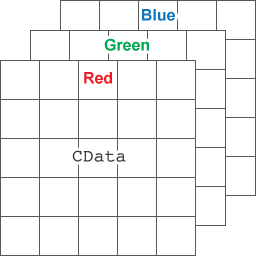
\includegraphics[width=0.2\linewidth]{./matrice_immagine.png}
\end{center}

Il primo indice viene usato per la coordinata $y$ ed il secondo per la coordinata $x$, con l'origine nel punto in alto a sinistra.
Dunque, $M(1,1,:)$ sarà un array monodimensionale che indica il colore del pixel in alto a sinistra.
\end{frame}

\begin{frame}{Immagini - colori}
Il colore di un punto viene descritto da un array di lunghezza 3 in quanto ogni colore può essere descritto come combinazione dei tre colori di base rosso verde e blu.

\centering
\begin{tabular}{|c|c|}
	\hline 
	Tripletta RGB & Colore \\ 
	\hline 
	1 0 0 & \textcolor{rosso}{Rosso} \\ 
	0 1 0 & \textcolor{verde}{Verde} \\ 
	0 0 1 & \textcolor{blu}{Blu} \\ 
	1 1 0 & \textcolor{giallo}{Giallo} \\ 
	1 0 1 & \textcolor{magenta}{Magenta} \\
	0 1 1 & \textcolor{ciano}{Ciano} \\ 
	0 0 0 & Nero \\ 
	1 1 1 & Bianco \\ 
	\hline 
\end{tabular} 
\end{frame}

\begin{frame}[fragile]{Immagini - Bandiera Italiana}
Creiamo un'immagine della bandiera italiana.
Dato che una bandiera ha un rapporto fra le dimensioni di 2:3 creiamo un'immagine con 200 pixel verticali e 300 pixel orizzontali:
\begin{lstlisting}[style=matlab]
bandiera = zeros(200,300,3);
\end{lstlisting}

E dipingiamo le tre bande verticali di verde, bianco e rosso:
\begin{lstlisting}[style=matlab, firstnumber=2]
bandiera(:, 1:100, 2) = 1;
bandiera(:, 101:200, :) = 1;
bandiera(:, 201:300, 1) = 1;
\end{lstlisting}

E mostriamo la figura:
\begin{lstlisting}[style=matlab, firstnumber=5]
imagesc(bandiera);
\end{lstlisting}
\end{frame}

\begin{frame}[allowframebreaks]{Competizione bandiere}
Quest'anno avete l'opportunità di guadagnare punti extra all'esame con delle competizioni.

La prima competizione riguarda proprio la creazione di una bandiera. Dovrete scrivere del codice matlab che crei l'immagine di una bandiera secondo le seguenti regole:
\begin{enumerate}
	\item Area minima di 200x500 pixel
	\item La bandiera deve essere realizzata interamente con uno script MATLAB, senza interazione con l'utente
	\item È necessario usare operazioni vettoriali, si possono usare cicli
	\item Verrà valutata sia l'estetica della bandiera, sia la struttura del codice utilizzato per realizzarla
	\item Potete presentare una sola bandiera a persona
	\item È necessario caricare nella cartella delle consegne (su beep, corso \emph{Competitions Informatica B}) un file .zip contenente la bandiera (un'immagine .png) e lo script che la genera, opportunamente indentato e commentato. Nel commento in testa al file specificate il vostro nome, cognome, numero di matricola e il vostro docente di Informatica B. È necessario rispettare la scadenza indicata (1/12/2018 ore 23.59).
\end{enumerate}

Verrà assegnato un punto all'esame per il primo classificato/la prima classificata di ogni scaglione.

Iscrivetevi (in beep) al corso \emph{Competitions Informatica B}.

Come disegnare una buona bandiera:
\begin{itemize}
\item \href{https://www.youtube.com/watch?v=BRNzeiV14bY}{The Big Bang Theory - Fun with Flags}
\item \href{https://www.youtube.com/watch?v=pnv5iKB2hl4}{Why city flags may be the worst-designed thing you've never noticed | Roman Mars}
\end{itemize}
\end{frame}

\begin{frame}{Rotazione di matrice}
Sc scriva una script in Matlab/Octave che data una matrice $a$ di dimensioni $N\times N$ crea una nuova matrice $b$ ruotata di 90 gradi in senso antiorario rispetto ad $a$.

Si consideri $N=4$ e la matrice $a$ inizializzata con i valori:

\centering
\begin{tabular}{|cccc|}
	\hline
	1&2&3&4\\
	2&3&4&5\\
	6&7&8&9\\
	0&0&0&0\\
	\hline
\end{tabular}
\end{frame}

\begin{frame}{Sequenza palindroma}
Si scriva uno script che chiede l’inserimento di una sequenza di N numeri e alla fine dice se la sequenza è palindroma o no.

Si ricorda che una sequenza è palindroma se risulta uguale letta da sinistra verso destra o da destra verso sinistra
\end{frame}

\begin{frame}{Confronti}
Si scriva uno script che chiede di inserire una sequenza di N numeri.

Successivamente, si inserisca un ulteriore numero e si dica se tutti i numeri della sequenza sono minori, uguali o maggiori di tale numero.
\end{frame}

\begin{frame}{Confronti con matrici}
Scrivere in Matlab uno script che, data una matrice $m$ di numeri, restituisce in uscita una matrice $mr$, ottenuta da $m$ nel seguente modo:
\begin{itemize}
	\item si calcola la media aritmetica dei valori di $m$;
	\item per i valori che in $m$ sono minori della media, in $m$r si
pone nella stessa posizione il valore -1, per quelli superiori alla media si pone il valore 1, e per gli altri (quelli uguali alla media) si pone lo stesso valore.
\end{itemize}

Si utilizzi la seguente matrice $m$

\centering
\begin{tabular}{|ccc|}
	\hline
	-2&2&3\\
	4&5&6\\
	\hline
\end{tabular}
\end{frame}

\begin{frame}{Inserimento ordinato nell'array}
Scrivere un programma che acquisisce da tastiera una serie di interi e li memorizza in modo ordinato nell'array.

\pause
Se, per esempio, $a = \{1, 3, 4, …\}$ e si vuole inserire 2, i valori 3 e 4 devono essere spostati a destra per fare spazio al nuovo elemento:

\centering
\begin{tabular}{|c|c|c|c|}
	\hline
	1&3&4&...\\
	\hline
\end{tabular}
$\rightarrow$
\begin{tabular}{|c|c|c|c|c|}
	\hline
	1& \alert{2} &3&4&...\\
	\hline
\end{tabular}

\end{frame}

\end{document}